\documentclass[tikz]{standalone}
\usepackage{tikz}
\usetikzlibrary{bayesnet}

\begin{document}
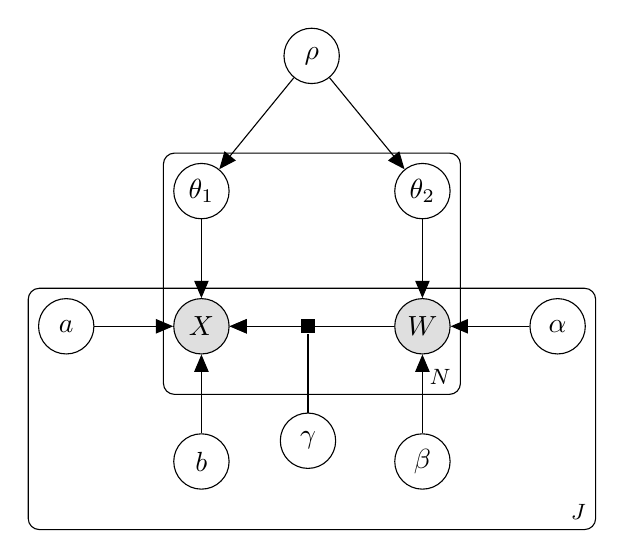
\begin{tikzpicture}
	\node[obs]	(X)	{$X$};
	\factor[right=of X, xshift=0.5cm]		{X-f}		{}	{}	{};
	\node[obs, right=of X-f]	(W)	{$W$};
	\node[latent, above=of X]	(theta1)	{$\theta_1$};
	\node[latent, above=of W]	(theta2)	{$\theta_2$};
	\node[latent, below=of X]		(b)		{$b$};
	\node[latent, left=of X]	(a)		{$a$};
	\node[latent, right=of W]	(alpha)		{$\alpha$};
	\node[latent, below=of W]		(beta)		{$\beta$};
	\node[latent, below=of X-f]	(gamma)		{$\gamma$};
	\node[latent, above=of theta1, xshift=1.4cm]	(rho)	{$\rho$};


	\edge 	{theta1}	{X};
	\edge	{theta2}	{W};
	\edge	{rho}	{theta1};
	\edge	{rho}	{theta2};
	\edge	{a}		{X};
	\edge	{b}		{X};
	\edge	{alpha}		{W};
	\edge	{beta}		{W};
	\factoredge		{gamma}	{X-f}	{X};
	\factoredge		{W}		{X-f}	{X};

	\plate	{plate1}	{
		(theta1)(theta2)
		(X)(W)
	}{$N$}

	\plate  {plate2}	{
		(a)(alpha)
		(b)(beta)
	}{$J$}


\end{tikzpicture}
\end{document}